\part{Spring Boot}


\begin{frame}[t]{The Way towards Spring Boot}
\small
\begin{columns}[T] 
\begin{column}{.42\textwidth}
    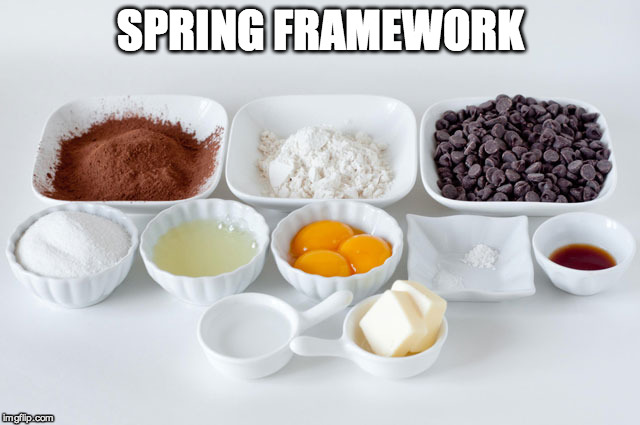
\includegraphics[width=\textwidth]{../SpringBoot/images/spring-ingredients}
\end{column}
\begin{column}{.55\textwidth}
\ldots Like the Individual Ingredients \ldots
    \begin{itemize}
    \item Full flexibility \& transparency: \\libraries, configuration, \ldots
    \item Some integration efforts
    \end{itemize}
\end{column}
\end{columns}
\vfill
\only<2>{
\begin{columns}[T] 
\begin{column}{.42\textwidth}
	
\includegraphics[width=\textwidth]{../SpringBoot/images/boot-cake}
\end{column}
\begin{column}{.55\textwidth}
\ldots Like the Ready-To-Bake Cake \ldots
	\begin{itemize}
		\item Simplified dependency management with starter packages
		\item Spring Auto Configuration %to remove boilerplate code and lower integration efforts w/o code generation
		\item Some uncertainties what's included
	\end{itemize}
\end{column}
\end{columns}
}
\end{frame}

\begin{frame}[t]{Spring Boot}
\begin{block}{Spring Boot \textit{by Pivotal Software \textsuperscript{\textcopyright}}}
	\begin{itemize}
	\item Simplifies Spring Cloud Application development
	\item Huge OS community: tutorials, code examples, troubleshoot support
	\item Integrates smoothly with \textbf{Spring Cloud} components
	\end{itemize}
\end{block}
\vfill
\only<2>{
\textbf{Spring Cloud} for implementing common patterns in distributed systems:
\footnotesize
\begin{itemize}
	\item (Cloud Foundry) Connectors (already used)
	\item Version controlled Configuration Management, e.g. \codealt{Spring Cloud Config}
	\item Service Discovery, e.g. \codealt{Eureka, Zookeeper, Consul}
	\item Instance based Routing and Load Balancing, e.g. \codealt{Zuul + Ribbon}
	\item Distributed Tracing, e.g. \codealt{Sleuth or Zipkin}
	\item Distributed Messaging, e.g. \codealt{Spring Cloud Bus, Stream}
\end{itemize}
}	
\end{frame}


\begin{frame}[c]{Spring Boot - Getting Started}
\centerline{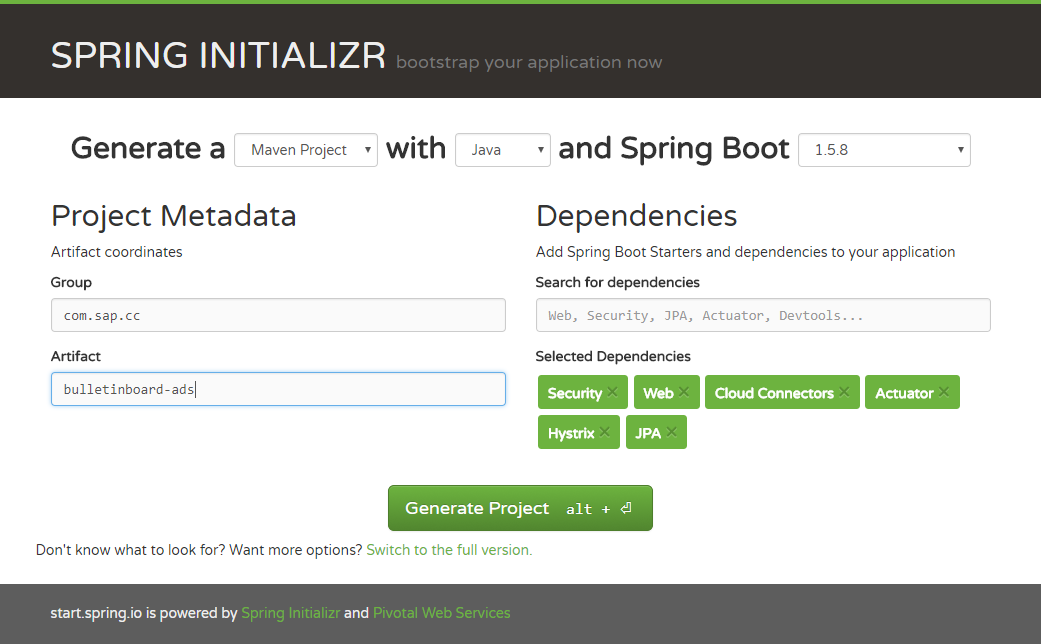
\includegraphics[width=0.8\textwidth]{../SpringBoot/images/Spring_Initializer}}
\centerline{\colorlink{https://start.spring.io/}{https://start.spring.io/}}
\vfill
\scriptsize
Spring Boot projects can also be created via \codealt{Spring Tool Suite} (Eclipse based IDE) or \codealt{IntelliJ}.
\end{frame}


\begin{frame}{The Magic of Spring Boot}{Convention over Configuration\footnote{without code generation and XML configuration}} 
\begin{description}
	\item['Starter' Project Object Models (POMs)] Third-party libraries and \textit{versions} are predefined to simplify Maven configuration.
\end{description}
\uncover<2>{\textbf{Example:} JPA Starter POM (\codealt{spring-boot-starter-data-jpa}) \\comes with \codealt{Hibernate} as default JPA implementation.}
\vfill
\begin{description}
	\item[Spring Auto Configuration] Tries to configure Spring automatically to reduce boilerplate code and lower integration efforts.
\end{description}
\uncover<2>{\textbf{Example:} If there is \codealt{H2} on the class path and no \codealt{DataSource} bean is configured then \codealt{H2} as embedded database is auto-configured.}
\end{frame}

\begin{frame}[t,fragile]{Demystify Spring Boot Magic: Starter POMs}
\footnotesize
\begin{block}{Parent POMs}
\begin{lstlisting}[language=xml,belowskip=-3mm,aboveskip=0mm]
<parent> <!-- has "spring-boot-dependencies" as parent that specifies versions -->
    <groupId>org.springframework.boot</groupId>
    <artifactId>spring-boot-starter-parent</artifactId>
    <version>1.5.3.RELEASE</version> 
</parent>
\end{lstlisting}
\end{block}
\begin{block}{Starter POMs}
\begin{lstlisting}[language=xml,belowskip=-3mm,aboveskip=0mm]
<dependency> <!-- contains necessary Spring Auto Configuration in version 1.5.3 -->
    <groupId>org.springframework.boot</groupId>
    <artifactId>spring-boot-starter</artifactId>
</dependency>
<dependency> <!-- contains necessary JPA / Hibernate dependencies -->
    <groupId>org.springframework.boot</groupId>
    <artifactId>spring-boot-starter-data-jpa</artifactId>
</dependency>
\end{lstlisting}
\end{block}
Note: The Spring Boot version needs to be specified once (in the \code{<parent>} section) and not for each Starter POM.
\end{frame}



\begin{frame}[t,fragile]{Demystify Spring Boot Magic: Auto Configuration}{How is it enabled for your application?}
\begin{block}{Application Entry Point}
\begin{lstlisting}[language=java,belowskip=-3mm,aboveskip=0mm]
// This class should be the primary \codealt{@Configuration} class. 
@SpringBootApplication
public class MyApplication {

    public static void main(String[] args) {
        SpringApplication.run(MyApplication.class, args);
    }
}
\end{lstlisting}
\end{block}
\vfill
\small
\textbf{\codealt{@SpringBootApplication}} is comprised of the annotations: \\\codealt{@Configuration}, \codealt{@ComponentScan} and \textbf{\codealt{@EnableAutoConfiguration}}. 
\vfill
\textbf{\codealt{SpringApplication}} bootstraps your application: \\creates Spring \codealt{ApplicationContext} and exposes command line arguments as Spring properties.
\end{frame}
    
\begin{frame}[t,fragile]{Demystify Spring Boot Magic: Auto Configuration}{How decisions are made?}
\small
\textbf{\codealt{@EnableAutoConfiguration}} configures \codealt{ApplicationContext} depending on presence / absence of \ldots
\begin{itemize}
	\item classes found on the classpath (Maven dependencies)
	\item beans defined by the application
	\item properties and other \colorlink{https://docs.spring.io/spring-boot/docs/current/api/org/springframework/boot/autoconfigure/condition/package-summary.html}{@Conditional annotations}
\end{itemize}
\begin{visibleenv}<2->
\begin{block}{Extract from \colorlink{https://github.com/spring-projects/spring-boot/blob/v1.5.8.RELEASE/spring-boot-autoconfigure/src/main/java/org/springframework/boot/autoconfigure/amqp/RabbitAutoConfiguration.java}{\codealt{RabbitAutoConfiguration}}}
\begin{lstlisting}[language=java,belowskip=-4mm,aboveskip=-1mm]
@Configuration
@ConditionalOnClass({RabbitTemplate.class, Channel.class})
@EnableConfigurationProperties(RabbitProperties.class)
public class RabbitAutoConfiguration {

    @Configuration
    @ConditionalOnMissingBean(RestTemplate.class)
    protected static class RabbitTemplateCreator {
        //executed when RabbitTemplate is on class path but there is no Bean
    }
}
\end{lstlisting}
\end{block}
\end{visibleenv}
\end{frame}

\begin{frame}[fragile]{Auto Configuration Report (/autoconfig)}
	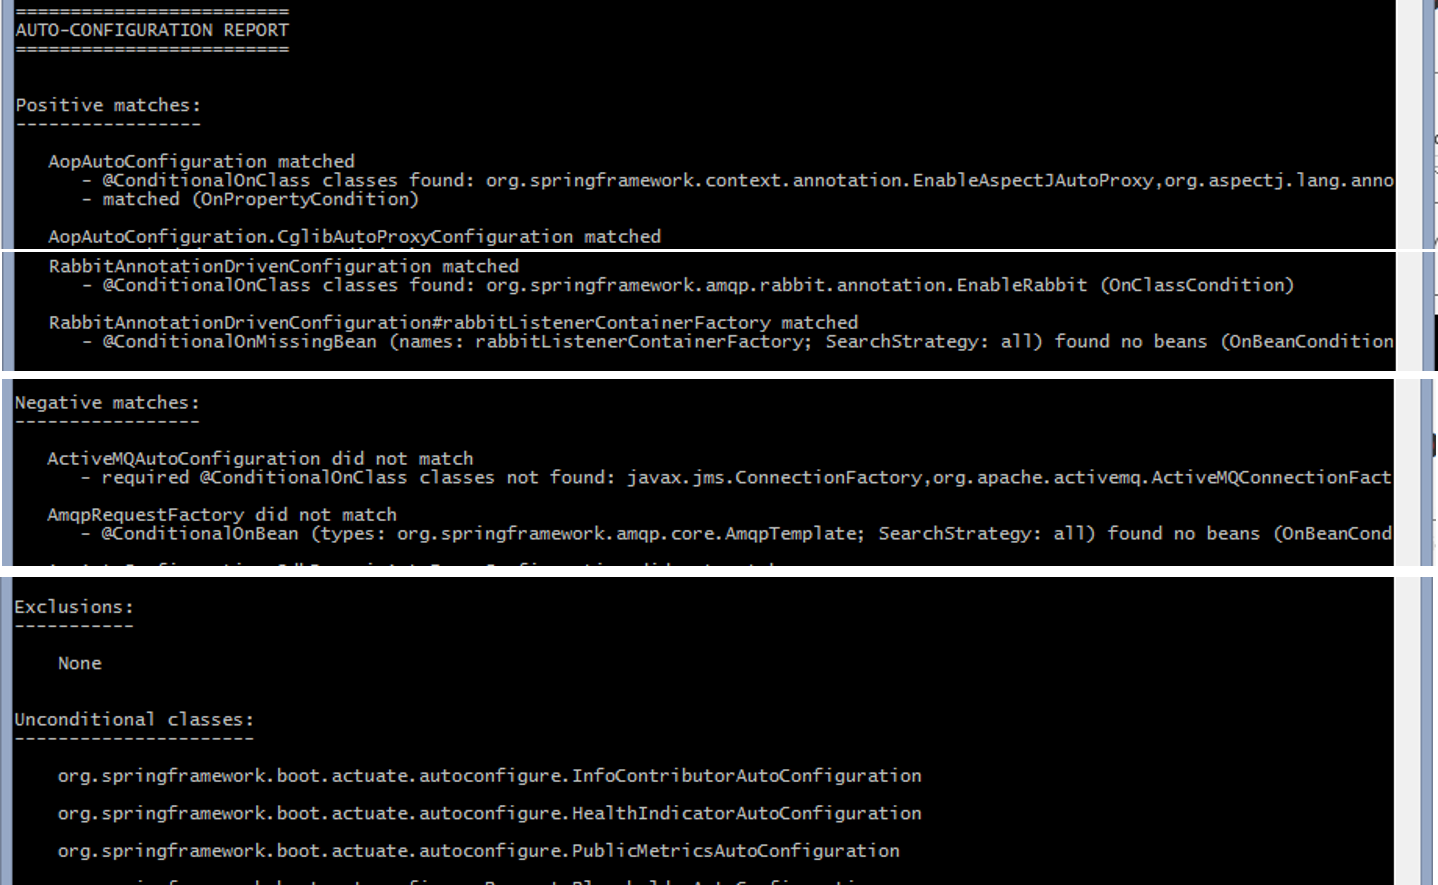
\includegraphics[trim=10 400 30 0,clip,width=\textwidth]{../SpringBoot/images/SpringBoot_AutoConfigurationReport}
\vfill
\textbf{Report shows config conditions for all components}
\footnotesize
\begin{itemize}
	\item Positive Matches: condition matches -> do config
	\item Negative Matches: no match -> do nothing
	\item Exclusions (explicitly defined by you)
	\item Unconditional classes -> always configured, no conditions
\end{itemize}

\begin{block}{Enable e.g. via command line argument}
\begin{lstlisting}[language=java,belowskip=-4mm,aboveskip=-1mm]
java -jar target/myproject-0.0.1-SNAPSHOT.jar --debug
\end{lstlisting} 
\end{block}
\vfill
\end{frame}


\begin{frame}[fragile]{Easily Change Spring Boot Defaults}
\footnotesize 
1. Specify \colorlink{https://docs.spring.io/spring-boot/docs/current/reference/html/common-application-properties.html}{properties} to tune/disable configuration, e.g. \codealt{spring.jmx.enabled=false}.
\vfill
\begin{visibleenv}<2->
2. Gradually replace auto configuration
\begin{itemize}
	\item Add other dependencies into \codealt{pom.xml} and/or define your own Beans.
	\item Exclude auto configuration classes, e.g.:
		\begin{lstlisting}[language=java]
@SpringBootApplication(exclude={SomeAutoConfiguration.class})
public class MyApplication {
}
		\end{lstlisting}
\end{itemize}
\end{visibleenv}
\begin{visibleenv}<3->
3. Exclude particular dependencies from Starter POM e.g. when replacing	Hibernate with EclipseLink.
		\begin{lstlisting}[language=xml]	
<dependency>
    <groupId>org.springframework.boot</groupId>
    <artifactId>spring-boot-starter-data-jpa</artifactId>
    <exclusions> ... </exclusions>
</dependency>
		\end{lstlisting}
\end{visibleenv}
\begin{visibleenv}<4->
4. Write your own custom Auto Configuration as documented \colorlink{https://docs.spring.io/spring-boot/docs/current/reference/html/boot-features-developing-auto-configuration.html\#boot-features-custom-starter-module-autoconfigure}{here}.
\end{visibleenv}
\end{frame}

\begin{frame}{Typical Use Cases for Tuning Auto Configuration}
\begin{itemize}
	\item You want to \textit{exclude} a default component that you do not use at all (save resources).
	\item You want to \textit{prevent} that a component is used in production \\e.g. embedded database.
	\item You want to configure \textit{environment specific behavior} \\e.g. for testing purposes.
	\item You want to \textit{add} your own component and specify default configuration and integration with other components.
\end{itemize}
\end{frame}

\begin{frame}[fragile]{Cascading Resolution of Property Sources}{Use Profiles to specify environment specific property values}
\footnotesize
\textbf{Property sources are considered in the following precedence (high to low):}
\begin{itemize}
	\item Command line arguments
	\item Servlet environment
	\item System environment variables
	\item \codealt{application-\{profile\}.properties} for \textbf{environment specific property values}\footnote{\scriptsize Override \codealt{default} profile with \codealt{spring.profiles.active} property or \codealt{@ActiveProfiles}.}
	\item \codealt{application.properties} (and YAML variants)
\end{itemize}
\begin{visibleenv}<2->
\begin{block}{Inject properties using \codealt{@Value} annotation}
\begin{lstlisting}[language=java,belowskip=-4mm,aboveskip=-1mm]
@Component
public class MyBean {

    @Value("${sap.com.cc.property}")
    private String property;
}
\end{lstlisting}
\end{block}
Property values can also be bound to structured objects via \colorlink{https://docs.spring.io/spring-boot/docs/current/reference/html/boot-features-external-config.html\#boot-features-external-config-typesafe-configuration-properties}{\codealt{@ConfigurationProperties}}.
\end{visibleenv}
\end{frame}

%\begin{frame}{Packaging options - JAR or WAR}
%\end{frame}


\begin{frame}{Further References}
\begin{itemize}
\item \colorlink{https://github.com/ccjavadev/cc-coursematerial/blob/master/SpringBoot/Readme.md}{Additional Notes: Further Differences}

\item \colorlink{https://docs.spring.io/spring-boot/docs/current/reference/pdf/spring-boot-reference.pdf}{Spring Boot Reference (PDF)}

\item \colorlink{https://docs.spring.io/spring-boot/docs/current/reference/html/common-application-properties.html}{Common Application Properties}

\item \colorlink{https://docs.spring.io/spring-boot/docs/current/reference/html/auto-configuration-classes.html}{Auto Configuration classes}

\item \colorlink{https://spring.io/guides}{Spring (Boot) tutorials}

\item \colorlink{https://github.wdf.sap.corp/d022051/SpringTutorial/wiki}{SAP internal Spring (Boot) Tutorial}

\item \colorlink{https://docs.spring.io/spring-boot/docs/current/reference/html/howto-spring-boot-application.html\#howto-troubleshoot-auto-configuration}{Troubleshoot Auto Configuration}
\end{itemize}
\end{frame}
